\section{Stato dell'arte dei moduli PPG}
\textcolor{red}{introduzione}

\textbf{MAX86916} Il modulo MAX86916 è un sensore ottico integrato per applicazioni di bio-sensing, prossimità e colore\cite{IntegratedMAX86916}\todo{definizione dal datasheet: da discutere}. Include quattro LED (rosso, infrarosso, verde, blu), un fotodiodo, elementi ottici e elettronica a basso rumore per circuiti di rimozione della luce ambientale. Il sensore è progettato per agevolare l'utilizzo in dispositivi indossabili, smartphone e assistenti per il fitness. Infatti presenta dimensioni molto ridotte (3.5mm x 7.0 mm x 1.5 mm) e bassi consumi. Il modulo utilizza una singola alimentazione da 1.8 V e un'alimentazione separata di 5.5 V per i LED interni. \`E possibile comunicare con il modulo attraverso un'interfaccia standard I\ap{2}C. Spesso è utilizzato per misurazioni di frequenza cardiaca, saturazione di ossigeno e piattaforme di sensori bio-ottici in modalità riflessiva. Presenta un ADC a 19 bit con frequenza di campionamento programmabile da 50 Hz a 3200 Hz. Il dispositivo integra anche una funzione di prossimità che permette di ridurre la luce visibile e i consumi quando non rileva una superficie vicina. Inoltre, grazie alla presenza di un \textit{Ambient Light Cancellation} (ALC) e di un \textit{Cross Talk Cancellation} è possibile ridurre gli errori di misura causati dall'interferenza della luce ambientale e degli elementi ottici usati.
\begin{figure}[h]
	\centering
	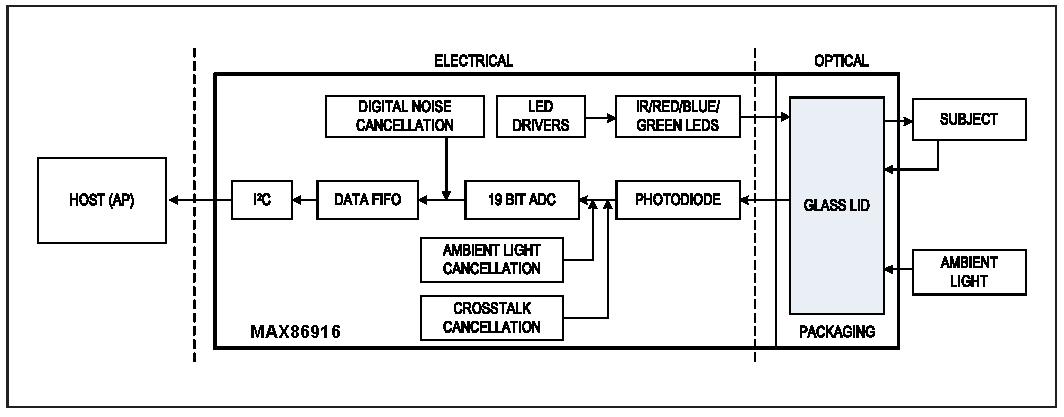
\includegraphics[width=1\linewidth]{ImageFiles/Fotopletismografia/MAX86916BlockDiagram}
	\caption{Schema a blocchi del modulo MAX86916.}
	\label{fig:MAX86916BlockDiagram}
\end{figure}

\textbf{MAX86916}
\begin{figure}[h]
	\centering
	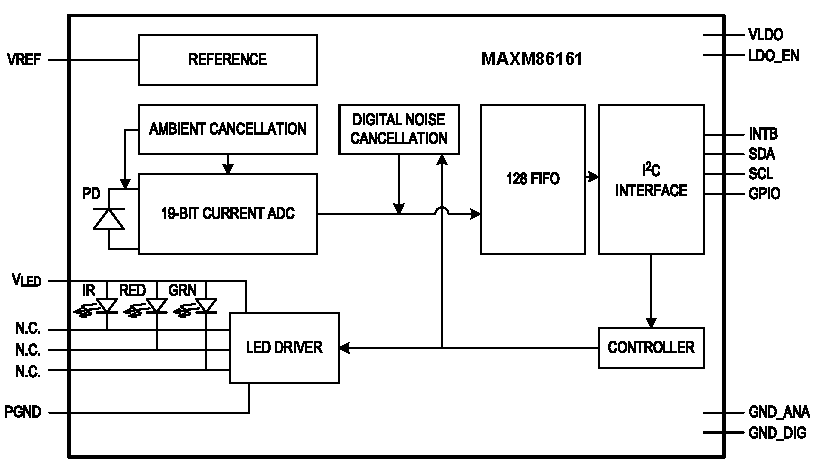
\includegraphics[width=0.9\linewidth]{ImageFiles/Fotopletismografia/MAXM86161BlockDiagram}
	\caption{Schema a blocchi del modulo MAXM86161.}
	\label{fig:MAXM86161BlockDiagram}
\end{figure}

